% move all configuration stuff into includes file so we can focus on the content
\documentclass[aspectratio=169,hyperref={pdfpagelabels=false,colorlinks=true,linkcolor=white,urlcolor=blue},t]{beamer}

%%%%%%%%%%%%%%%%%%%%%%%%%%%%%%%%%%%%%%%%%%%%%%%%%%%%%%%%%%%%%%%%%%%%%%%%%%%%%%%%%%
%%%%%%%%%%%%%%%%%%%%%%%%%%%%%%%%%%%%%%%%%%%%%%%%%%%%%%%%%%%%%%%%%%%%%%%%%%%%%%%%%%
% packages
\usepackage{pict2e}
\usepackage{epic}
\usepackage{amsmath,amsfonts,amssymb}
\usepackage{units}
\usepackage{fancybox}
\usepackage[absolute,overlay]{textpos} 
\usepackage{media9} % avi2flv: "C:\Program Files\ffmpeg\bin\ffmpeg.exe" -i TuneFreqFilterbank.avi -b 600k -s 441x324 -r 15 -acodec copy TuneFreqFilterbank.flv
\usepackage{animate}
\usepackage{gensymb}
\usepackage{multirow}
\usepackage{silence}
\usepackage{tikz}
\usepackage[backend=bibtex,style=ieee]{biblatex}
\AtEveryCitekey{\iffootnote{\tiny}{}}
\addbibresource{include/references}

%%%%%%%%%%%%%%%%%%%%%%%%%%%%%%%%%%%%%%%%%%%%%%%%%%%%%%%%%%%%%%%%%%%%%%%%%%%%%%%%%%
%%%%%%%%%%%%%%%%%%%%%%%%%%%%%%%%%%%%%%%%%%%%%%%%%%%%%%%%%%%%%%%%%%%%%%%%%%%%%%%%%%
% relative paths
\graphicspath{{graph/}}


%%%%%%%%%%%%%%%%%%%%%%%%%%%%%%%%%%%%%%%%%%%%%%%%%%%%%%%%%%%%%%%%%%%%%%%%%%%%%%%%%%
%%%%%%%%%%%%%%%%%%%%%%%%%%%%%%%%%%%%%%%%%%%%%%%%%%%%%%%%%%%%%%%%%%%%%%%%%%%%%%%%%%
% units
\setlength{\unitlength}{1mm}

%%%%%%%%%%%%%%%%%%%%%%%%%%%%%%%%%%%%%%%%%%%%%%%%%%%%%%%%%%%%%%%%%%%%%%%%%%%%%%%%%%
%%%%%%%%%%%%%%%%%%%%%%%%%%%%%%%%%%%%%%%%%%%%%%%%%%%%%%%%%%%%%%%%%%%%%%%%%%%%%%%%%%
% theme & layout
\usetheme{Frankfurt}
\beamertemplatenavigationsymbolsempty
%\setbeamertemplate{frametitle}[smoothbars theme]
\setbeamertemplate{frametitle}
{
    \begin{beamercolorbox}[ht=1.8em,wd=\paperwidth]{frametitle}
        \vspace{-.1em}%
        \hspace{.2em}{\strut\insertframetitle\strut}
        
        \hspace{.2em}\small\strut\insertframesubtitle\strut
        %\hfill
        %\includegraphics[height=.8cm,keepaspectratio]{CenterMusicTechnology-solid-2lines-white-CoAtag}
        
    \end{beamercolorbox}
    \begin{textblock*}{100mm}(11.6cm,.7cm)
        \includegraphics[height=.8cm,keepaspectratio]{Logo_GTCMT_black}
    \end{textblock*}
}
\setbeamertemplate{footline}[frame number]

% set this to ensure bulletpoints without subsections
\usepackage{remreset}
\makeatletter
\@removefromreset{subsection}{section}
\makeatother
\setcounter{subsection}{1}

%---------------------------------------------------------------------------------
% appearance
\setbeamercolor{structure}{fg=gtgold}
\setbeamercovered{transparent} %invisible
\setbeamercolor{bibliography entry author}{fg=black}
\setbeamercolor*{bibliography entry title}{fg=black}
\setbeamercolor*{bibliography entry note}{fg=black}
\setbeamercolor{frametitle}{fg=black}
\setbeamercolor{title}{fg=black}

%\usepackage{pgfpages}
%\setbeameroption{show notes}
%\setbeameroption{show notes on second screen=right}
%---------------------------------------------------------------------------------
% fontsize
\let\Tiny=\tiny

%%%%%%%%%%%%%%%%%%%%%%%%%%%%%%%%%%%%%%%%%%%%%%%%%%%%%%%%%%%%%%%%%%%%%%%%%%%%%%%%%%
%%%%%%%%%%%%%%%%%%%%%%%%%%%%%%%%%%%%%%%%%%%%%%%%%%%%%%%%%%%%%%%%%%%%%%%%%%%%%%%%%%
% warnings
\pdfsuppresswarningpagegroup=1
\WarningFilter{biblatex}{Patching footnotes failed}
\WarningFilter{latexfont}{Font shape}
\WarningFilter{latexfont}{Some font shapes}
\WarningFilter{gensymb}{Not defining}


%%%%%%%%%%%%%%%%%%%%%%%%%%%%%%%%%%%%%%%%%%%%%%%%%%%%%%%%%%%%%%%%%%%%%%%%%%%%%%%%%%
%%%%%%%%%%%%%%%%%%%%%%%%%%%%%%%%%%%%%%%%%%%%%%%%%%%%%%%%%%%%%%%%%%%%%%%%%%%%%%%%%%
% theme & layout
\usetheme{Frankfurt}
\useinnertheme{rectangles}


%%%%%%%%%%%%%%%%%%%%%%%%%%%%%%%%%%%%%%%%%%%%%%%%%%%%%%%%%%%%%%%%%%%%%%%%%%%%%%%%%%
\setbeamertemplate{frametitle}[default][colsep=-4bp,rounded=false,shadow=false]
\setbeamertemplate{frametitle}
{%
    \nointerlineskip%
    %\vskip-0.5ex
    \begin{beamercolorbox}[wd=\paperwidth,ht=3.5ex,dp=0.6ex]{frametitle}
        \hspace*{1.3ex}\insertframetitle%
        
        \hspace*{1.3ex}\small\insertframesubtitle%
    \end{beamercolorbox}%
    \begin{textblock*}{100mm}(11.6cm,.57cm)
        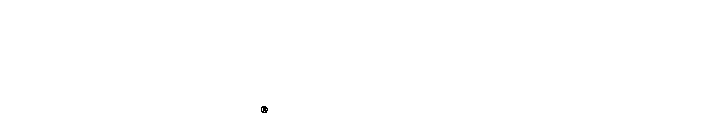
\includegraphics[height=.8cm,keepaspectratio]{graph/Logo_GTCMT_white}
    \end{textblock*}
}


%%%%%%%%%%%%%%%%%%%%%%%%%%%%%%%%%%%%%%%%%%%%%%%%%%%%%%%%%%%%%%%%%%%%%%%%%%%%%%%%%%
\setbeamertemplate{title page}[default][colsep=-4bp,rounded=false,shadow=false]
\setbeamertemplate{title page}
{
    \begin{textblock*}{100mm}(15cm,.51cm)
            \href{https://github.com/alexanderlerch/ACA-Slides/blob/2nd_edition/\jobname.pdf}{\includegraphics[height=.5cm,keepaspectratio]{graph/Logo_github}}\hspace*{2ex}
    \end{textblock*}
    \vskip-10ex
    \begin{beamercolorbox}[wd=\paperwidth,ht=.7\paperheight,dp=0.6ex]{frametitle} %35ex
        %\begin{flushright}
            %\href{http://www.gtcmt.gatech.edu}{\includegraphics[height=.8cm,keepaspectratio]{graph/Logo_GTCMT_black}}\hspace*{2ex}
        %\end{flushright}
        
        \hspace*{1.8ex}\LARGE\inserttitle%
        
        \vspace*{.5ex}
        
        \hspace*{1.3ex}\small\insertsubtitle%
        
        \vspace*{.5ex}
    \end{beamercolorbox}%
    \nointerlineskip%
    \begin{beamercolorbox}[wd=\paperwidth,ht=.4\paperheight,dp=0.6ex]{page number in head/foot}
        %\vspace*{-.5ex}
        \hspace*{1.7ex}\small\insertauthor%
        
        %\hspace*{1.7ex}\small }%
        
        \vspace*{10ex}
        
        \begin{flushright}
            \href{http://www.gtcmt.gatech.edu}{\includegraphics[height=.8cm,keepaspectratio]{graph/Logo_GTCMT_black}}\hspace*{2ex}
        \end{flushright}
    \end{beamercolorbox}%
}


%%%%%%%%%%%%%%%%%%%%%%%%%%%%%%%%%%%%%%%%%%%%%%%%%%%%%%%%%%%%%%%%%%%%%%%%%%%%%%%%%%
%\makeatother
\setbeamertemplate{footline}
{
  \leavevmode%
  \hbox{%
  \begin{beamercolorbox}[wd=.5\paperwidth,ht=2.25ex,dp=1ex,left,leftskip=1ex]{page number in head/foot}%
    \insertsubtitle
  \end{beamercolorbox}%
  \begin{beamercolorbox}[wd=.5\paperwidth,ht=2.25ex,dp=1ex,right,rightskip=1ex]{page number in head/foot}%
    \hfill
    \insertframenumber{} / \inserttotalframenumber
  \end{beamercolorbox}}%
  \vskip0pt%
}
%\makeatletter


%%%%%%%%%%%%%%%%%%%%%%%%%%%%%%%%%%%%%%%%%%%%%%%%%%%%%%%%%%%%%%%%%%%%%%%%%%%%%%%%%%
\beamertemplatenavigationsymbolsempty
\setbeamertemplate{navigation symbols}{}
\setbeamertemplate{blocks}[default]%[rounded=false,shadow=false]
\setbeamertemplate{itemize item}[square]
\setbeamertemplate{itemize subitem}[circle]
\setbeamertemplate{itemize subsubitem}[triangle]
\setbeamertemplate{enumerate item}[square]
\setbeamertemplate{enumerate subitem}[circle]
\setbeamertemplate{enumerate subsubitem}[circle]


%%%%%%%%%%%%%%%%%%%%%%%%%%%%%%%%%%%%%%%%%%%%%%%%%%%%%%%%%%%%%%%%%%%%%%%%%%%%%%%%%%
% colors
\setbeamercolor{structure}{fg=darkgray}
\setbeamercovered{transparent} %invisible
\setbeamercolor{bibliography entry author}{fg=black}
\setbeamercolor*{bibliography entry title}{fg=black}
\setbeamercolor*{bibliography entry note}{fg=black}
\setbeamercolor{frametitle}{fg=black}
\setbeamercolor{title}{fg=white}
\setbeamercolor{subtitle}{fg=white}
\setbeamercolor{frametitle}{fg=white}
\setbeamercolor{framesubtitle}{fg=white}
\setbeamercolor{mini frame}{fg=white, bg=black}
\setbeamercolor{section in head/foot}{fg=white, bg=darkgray}
\setbeamercolor{page number in head/foot}{fg=black, bg=lightblue}
\setbeamercolor{item projected}{fg=white, bg=black}

%---------------------------------------------------------------------------------
%%%%%%%%%%%%%%%%%%%%%%%%%%%%%%%%%%%%%%%%%%%%%%%%%%%%%%%%%%%%%%%%%%%%%%%%%%%%%%%%%%
%%%%%%%%%%%%%%%%%%%%%%%%%%%%%%%%%%%%%%%%%%%%%%%%%%%%%%%%%%%%%%%%%%%%%%%%%%%%%%%%%%
% title information
\title[]{Introduction to \textbf{Audio Content Analysis}}   
\author[alexander lerch]{alexander lerch} 
%\institute{~}
%\date[Alexander Lerch]{}
%\titlegraphic{\vspace{-16mm}\includegraphics[width=\textwidth,height=3cm]{title}}

%%%%%%%%%%%%%%%%%%%%%%%%%%%%%%%%%%%%%%%%%%%%%%%%%%%%%%%%%%%%%%%%%%%%%%%%%%%%%%%%%%
%%%%%%%%%%%%%%%%%%%%%%%%%%%%%%%%%%%%%%%%%%%%%%%%%%%%%%%%%%%%%%%%%%%%%%%%%%%%%%%%%%
% colors
\definecolor{gtgold}{HTML}{E0AA0F} %{rgb}{0.88,0.66,1,0.06} [234, 170, 0]/256
\definecolor{darkgray}{rgb}{.1, .1, .25}
\definecolor{lightblue}{rgb}{.1, 0.75, 1}
\definecolor{highlight}{rgb}{0, 0, 1} %_less!40

%%%%%%%%%%%%%%%%%%%%%%%%%%%%%%%%%%%%%%%%%%%%%%%%%%%%%%%%%%%%%%%%%%%%%%%%%%%%%%%%%%
%%%%%%%%%%%%%%%%%%%%%%%%%%%%%%%%%%%%%%%%%%%%%%%%%%%%%%%%%%%%%%%%%%%%%%%%%%%%%%%%%%
% relative paths
\graphicspath{{../ACA-Plots/graph/}}


%%%%%%%%%%%%%%%%%%%%%%%%%%%%%%%%%%%%%%%%%%%%%%%%%%%%%%%%%%%%%%%%%%%%%%%%%%%%%%%%%%
%%%%%%%%%%%%%%%%%%%%%%%%%%%%%%%%%%%%%%%%%%%%%%%%%%%%%%%%%%%%%%%%%%%%%%%%%%%%%%%%%%
% units
\setlength{\unitlength}{1mm}

%%%%%%%%%%%%%%%%%%%%%%%%%%%%%%%%%%%%%%%%%%%%%%%%%%%%%%%%%%%%%%%%%%%%%%%%%%%%%%%%%%
%%%%%%%%%%%%%%%%%%%%%%%%%%%%%%%%%%%%%%%%%%%%%%%%%%%%%%%%%%%%%%%%%%%%%%%%%%%%%%%%%%
% math
\DeclareMathOperator*{\argmax}{argmax}
\DeclareMathOperator*{\argmin}{argmin}
\DeclareMathOperator*{\atan}{atan}
\DeclareMathOperator*{\arcsinh}{arcsinh}
\DeclareMathOperator*{\sign}{sign}
\DeclareMathOperator*{\tcdf}{tcdf}
\DeclareMathOperator*{\si}{sinc}
\DeclareMathOperator*{\princarg}{princarg}
\DeclareMathOperator*{\arccosh}{arccosh}
\DeclareMathOperator*{\hwr}{HWR}
\DeclareMathOperator*{\flip}{flip}
\DeclareMathOperator*{\sinc}{sinc}
\DeclareMathOperator*{\floor}{floor}
\newcommand{\e}{{e}}
\newcommand{\jom}{\mathrm{j}\omega}
\newcommand{\jOm}{\mathrm{j}\Omega}
\newcommand   {\mat}[1]    		{\boldsymbol{\uppercase{#1}}}		%bold
\renewcommand {\vec}[1]    		{\boldsymbol{\lowercase{#1}}}		%bold

%%%%%%%%%%%%%%%%%%%%%%%%%%%%%%%%%%%%%%%%%%%%%%%%%%%%%%%%%%%%%%%%%%%%%%%%%%%%%%%%%%
%%%%%%%%%%%%%%%%%%%%%%%%%%%%%%%%%%%%%%%%%%%%%%%%%%%%%%%%%%%%%%%%%%%%%%%%%%%%%%%%%%
% media9
\newcommand{\includeaudio}[1]{
\href{run:audio/#1.mp3}{
\includegraphics[width=5mm, height=5mm]{graph/SpeakerIcon}}}

\newcommand{\includeanimation}[4]{{\begin{center}
                        \animategraphics[autoplay,loop,scale=.7]{#4}{animation/#1-}{#2}{#3}        
                        \end{center}
                        \addreference{matlab source: \href{https://github.com/alexanderlerch/ACA-Plots/blob/master/matlab/animate#1.m}{matlab/animate#1.m}}}
                        \inserticon{video}}
                        
%%%%%%%%%%%%%%%%%%%%%%%%%%%%%%%%%%%%%%%%%%%%%%%%%%%%%%%%%%%%%%%%%%%%%%%%%%%%%%%%%%
%%%%%%%%%%%%%%%%%%%%%%%%%%%%%%%%%%%%%%%%%%%%%%%%%%%%%%%%%%%%%%%%%%%%%%%%%%%%%%%%%%
% other commands
\newcommand{\question}[1]{%\vspace{-4mm}
                          \setbeamercovered{invisible}
                          \begin{columns}[T]
                            \column{.9\textwidth}
                                \textbf{#1}
                            \column{.1\textwidth}
                                \vspace{-8mm}
                                \begin{flushright}
                                     
\includegraphics[width=.9\columnwidth]{graph/question_mark}
                                \end{flushright}
                                \vspace{6mm}
                          \end{columns}\pause\vspace{-12mm}}

\newcommand{\toremember}[1]{
                        \inserticon{lightbulb}
                        }

\newcommand{\matlabexercise}[1]{%\vspace{-4mm}
                          \setbeamercovered{invisible}
                          \begin{columns}[T]
                            \column{.8\textwidth}
                                \textbf{matlab exercise}: #1
                            \column{.2\textwidth}
                                \begin{flushright}
                                     \includegraphics[scale=.5]{graph/logo_matlab}
                                \end{flushright}
                                %\vspace{6mm}
                          \end{columns}}

\newcommand{\addreference}[1]{  
                  
                    \begin{textblock*}{\baselineskip }(.98\paperwidth,.5\textheight) %(1.15\textwidth,.4\textheight)
                         \begin{minipage}[b][.5\paperheight][b]{1cm}%
                            \vfill%
                             \rotatebox{90}{\tiny {#1}}
                        \end{minipage}
                   \end{textblock*}
                    }
                    
\newcommand{\figwithmatlab}[1]{
                    \begin{figure}
                        \centering
                        \includegraphics[scale=.7]{#1}
                        %\label{fig:#1}
                    \end{figure}
                    
                    \addreference{matlab source: \href{https://github.com/alexanderlerch/ACA-Plots/blob/main/matlab/plot#1.m}{plot#1.m}}}
\newcommand{\figwithref}[2]{
                    \begin{figure}
                        \centering
                        \includegraphics[scale=.7]{#1}
                        \label{fig:#1}
                    \end{figure}
                    
                    \addreference{#2}}  
                                    
\newcommand{\inserticon}[1]{
                    \begin{textblock*}{100mm}(14.5cm,7.5cm)
                        \includegraphics[height=.8cm,keepaspectratio]{graph/#1}
                    \end{textblock*}}            

%%%%%%%%%%%%%%%%%%%%%%%%%%%%%%%%%%%%%%%%%%%%%%%%%%%%%%%%%%%%%%%%%%%%%%%%%%%%%%%%%%
%%%%%%%%%%%%%%%%%%%%%%%%%%%%%%%%%%%%%%%%%%%%%%%%%%%%%%%%%%%%%%%%%%%%%%%%%%%%%%%%%%
% counters
\newcounter{i}
\newcounter{j}
\newcounter{iXOffset}
\newcounter{iYOffset}
\newcounter{iXBlockSize}
\newcounter{iYBlockSize}
\newcounter{iYBlockSizeDiv2}
\newcounter{iXBlockSizeDiv2}
\newcounter{iDistance}




\subtitle{Module 10.2: Audio-to-Audio \& Audio-to-Score Alignment}

%%%%%%%%%%%%%%%%%%%%%%%%%%%%%%%%%%%%%%%%%%%%%%%%%%%%%%%%%%%%%%%%%%%%%%%%%%%%
\begin{document}
    % generate title page
	{
\setbeamertemplate{headline}{} 
\setbeamertemplate{footline}{} 
\begin{frame}
    \titlepage
    %\vspace{-5mm}
\end{frame}
}
\addtocounter{framenumber}{-1}


    \section[overview]{lecture overview}
        \begin{frame}{introduction}{overview}
            \begin{block}{corresponding textbook section}
                    %\href{http://ieeexplore.ieee.org/xpl/articleDetails.jsp?arnumber=6331124}{Chapter 7: Alignment} (pp.~146--150)
                    sections~10.2 \& 10.3
            \end{block}

            \begin{itemize}
                \item   \textbf{lecture content}
                    \begin{itemize}
                        \item   Audio-to-Audio alignment
                            \begin{itemize}
                                \item   use cases
                                \item   features
                                \item   distance measures
                                \item   typical accuracy
                            \end{itemize}
                        \item   Audio-to-Score alignment
                    \end{itemize}
                \bigskip
                \item<2->   \textbf{learning objectives}
                    \begin{itemize}
                        \item   elaborate on possible use cases for audio-to-audio alignment
                        \item   give examples for features and distance measures for alignment
                        \item   discuss differences between audio-to-audio and audio-to-score alignment
                    \end{itemize}
            \end{itemize}
            \inserticon{directions}
        \end{frame}

    \section[A2A]{Audio to audio alignment}
        \begin{frame}{audio-to-audio alignment}{introduction}
            \begin{itemize}
                \item	\textbf{objective}
                    \begin{itemize}
                        \item	align two sequences of audio
                    \end{itemize}
                \bigskip
                \item<2->	\textbf{use cases}
                    \begin{itemize}
                        \item	\textit{quick browsing} for certain parts in recordings
                        \item	\textit{timing adjustment} (backing vocals, loops, \ldots)
                        \item	\textit{automated dubbing}
                        \item	\textit{musicological analysis} (relative timing of several performances)
                    \end{itemize}
                \bigskip
                \item<3->	\textbf{processing steps}
                    \begin{itemize}
                        \item	extract suitable features
                        \item	compute distance matrix
                        \item	compute alignment path
                    \end{itemize}
            \end{itemize}
        \end{frame}

        \begin{frame}{audio-to-audio alignment}{alignment path computation}
                 \vspace{-3mm}
           \begin{columns}
            \column{.4\linewidth}
            \vspace{4mm}
            \begin{itemize}
                \item prerequisite:\\ Module 10.1~---~Dynamic Time Warping
            \end{itemize}
            
            \column{.6\linewidth}
                \vspace{-13mm}
            \figwithmatlab{DtwPath}
            \end{columns}
        \end{frame}

        \begin{frame}{audio-to-audio alignment}{features}
            \vspace{-2mm}
            \only<1-2>{
                \begin{itemize}
                    \item	\textbf{use case examples}
                        \begin{itemize}
                            \item	\textbf{quick browsing} --- find the same part across files\\
                                $\Rightarrow$ use \textit{pitch based} features
                            \item	\textbf{timing adjustment} --- backing vocals to lead vocals\\
                                $\Rightarrow$ use \textit{intensity based} features
                            \item	\textbf{automated dubbing} --- same speaker several recordings\\
                                $\Rightarrow$ use \textit{intensity based} and \textit{timbre based} features
                        \end{itemize}
                    \smallskip
                    \item<2-> \textbf{feature categories}
                        \begin{itemize}
                            \item	\textbf{intensity}: energy, onset probability, \ldots
                            \item	\textbf{tonal}: pitch chroma, \ldots
                            \item	\textbf{timbral}: MFCCs, spectral shape, \ldots
                        \end{itemize}
                    \item<2->[] plot from \footfullcite{kirchhoff_evaluation_2011}
                \end{itemize}
            }
            \only<3>{
                \begin{figure}
                    \centerline{\includegraphics[scale=.5]{graph/ATAA_features}}
                \end{figure}
            }
        \end{frame}
        
        \begin{frame}{audio-to-audio alignment}{feature-dependency of results}
            \figwithmatlab{DtwFeatures}
            
            features (left to right): pitch chroma, RMS, MFCCs
        \end{frame}
        
        \begin{frame}{audio-to-audio alignment}{compute distance matrix --- distance measures}
            \begin{itemize}
                \item	typical distance measures
                    \only<1-4>{
                    \begin{itemize}
                        \item<1-4>	\emph{{Euclidean distance}}:
                                $d_\mathrm{E}(s) = \sqrt{\sum\limits_{j = 0}^{11}{\big(\nu_\mathrm{e}(j)-\nu_\mathrm{t,s}(j)\big)^2}} $
                        \item<2-4>	\emph{{Manhattan distance}}:
                                $d_\mathrm{M}(s) = \sum\limits_{j = 0}^{11}{\big|\nu_\mathrm{e}(j)-\nu_\mathrm{t,s}(j)\big|} $
                        \item<3-4>	\emph{{Cosine distance}}:
                                $d_\mathrm{C}(s) = 1-\left( \frac{\sum\limits_{j = 0}^{11}{\nu_\mathrm{e}(j)\cdot\nu_\mathrm{t,s}(j)}}{\sqrt{\sum\limits_{j = 0}^{11}{\nu_\mathrm{e}(j)^2}}\sqrt{\cdot \sum\limits_{j = 0}^{11}{\nu_\mathrm{t,s}(j)^2}}}\right) $
                        \item<4-4>	\emph{{Kullback-Leibler divergence}}:
                                $d_\mathrm{KL}(s) = \sum\limits_{j = 0}^{11}{\nu_\mathrm{e}(j)\cdot\log\left(\frac{\nu_\mathrm{e}(j)}{\nu_\mathrm{t,s}(j)}\right)}$
                    \end{itemize}
                    }
                \smallskip
                \item<5->	data-driven approach: train classifier with 2-class problem \footfullcite{kirchhoff_evaluation_2011}
                    \only<5>{
                        \begin{figure}
                            \centerline{\includegraphics[scale=.5]{graph/ATAA_feature_training}}
                        \end{figure}
                    }
                    \only<6>{
                        \begin{figure}
                            \centerline{\includegraphics[scale=.5]{graph/ATAA_simmatrix_compare}}
                        \end{figure}
                    }
            \end{itemize}
        \end{frame}
        
        \begin{frame}{audio-to-audio alignment}{typical results}
            \vspace{-5mm}
            \begin{columns}
            \column{.7\linewidth}
                \vspace{-3mm}\begin{figure}
                    \centerline{\includegraphics[width= \columnwidth]{graph/ATAA_results}}
                \end{figure}
            \column{.3\linewidth}
                \begin{table}
                    \begin{tabular}{p{.55\columnwidth}l}
                        \textbf{originals}\linebreak
                        \begin{scriptsize}
                            left:~instrumental\hfill \linebreak
                            right:~a capella
                        \end{scriptsize} & \textbf{synced}\\
                        \includeaudio{originals_splanky} & \includeaudio{synced_splanky}
                    
                    \end{tabular}
                \end{table}
            \end{columns}
            
            \hphantom{\footfullcite{kirchhoff_evaluation_2011}}
            \inserticon{audio}
        \end{frame}
        
    \section[A2S]{Audio to score alignment}
        \begin{frame}{audio-to-score alignment}{overview}
            \begin{itemize}
                \item   \textbf{objective}
                    \begin{itemize}
                        \item align an audio sequence with a score sequence
                    \end{itemize}
                \bigskip
                \item<2->   \textbf{use cases}
                    \begin{itemize}
                        \item   score viewer
                        \item   music education
                        \item   retrieve matching score/audio via cost function
                        \item   musicological analysis
                    \end{itemize}
                \bigskip
                \item<3->   \textbf{processing steps}
                    \begin{itemize}
                        \item   see audio-to-audio alignment
                    \end{itemize}
            \end{itemize}
        \end{frame}
        \begin{frame}{audio-to-score alignment}{challenges}
            \begin{itemize}
                \item   features from \textbf{different domains} 
                    \begin{itemize}
                    \item   score contains no timbre info
                    \item   score cannot be expected to contain no loudness info
                    \item   score has no clear ``time axis''
                    \end{itemize}
                \bigskip
                \item<2->[$\Rightarrow$]   two prototypical for distance/similarity calculation
                    \begin{itemize}
                        \item   \textit{approach 1}: convert score into audio-like representation
                            \begin{itemize}
                                \item   MIDI-to-audio
                                \item   use model synthesize
                            \end{itemize}
                        \smallskip
                        \item   \textit{approach 2}: convert audio into score-like representation
                            \begin{itemize}
                                \item   audio-to-MIDI 
                                \item   pitch chroma
                                \item   event-based segmentation
                            \end{itemize}
                    \end{itemize}
            \end{itemize}
        \end{frame}
    \section[eval]{evaluation}
        \begin{frame}{alignment}{evaluation}
            \begin{itemize}
                \item   \textbf{goal}: compare two sequences of time stamps
                \bigskip
                \item<2->   evaluation \textbf{challenges} 
                    \begin{itemize}
                    \item   pauses/rests, and long held notes: what is the reference path?
                    \item   noise in the begin and end of the recording
                    \item   data not easily available
                        \begin{itemize}
                            \item   synthesized
                            \item   piano sensors
                            \item   pseudo-ground truth with time stretching
                            \item   automatic annotation with quality assurance
                        \end{itemize}
                    \end{itemize}
             \end{itemize}
        \end{frame}
        \begin{frame}{alignment}{evaluation metrics}
            \begin{itemize}
                \item   \textit{audio-to-score}
                    \begin{itemize}
                        \item   missed note rate
                        \item   misalign rate
                        \item   piece completion
                        \item   average absolute deviation
                        \item   variance of deviation
                    \end{itemize}
                \bigskip
                \item   \textit{audio-to-audio}
                    \begin{itemize}
                        \item   mean deviation
                        \item   mean absolute deviation
                        \item   maximum deviation
                        \item   relative number of matching path points
                    \end{itemize}
            \end{itemize}
        \end{frame}

    
    \section{summary}
        \begin{frame}{summary}{lecture content}
            \begin{itemize}
                \item   \textbf{audio-to-audio alignment}
                    \begin{enumerate}
                        \item   extract features
                        \item   create distance matrix with suitable distance measure
                        \item   use DTW to find alignment path
                        \item   (use time-stretching to actually align the sequences)
                    \end{enumerate}
                \bigskip
                \item   \textbf{audio-to-score alignment}
                    \begin{enumerate}
                        \item   extract usually pitch-based features
                        \item   distance measure
                        \item   use DTW, HMM, etc to extract alignment path
                    \end{enumerate}
            \end{itemize}
            \inserticon{summary}
        \end{frame}
\end{document}
